\section{Implementation}

\begin{figure}
  \begin{center}
    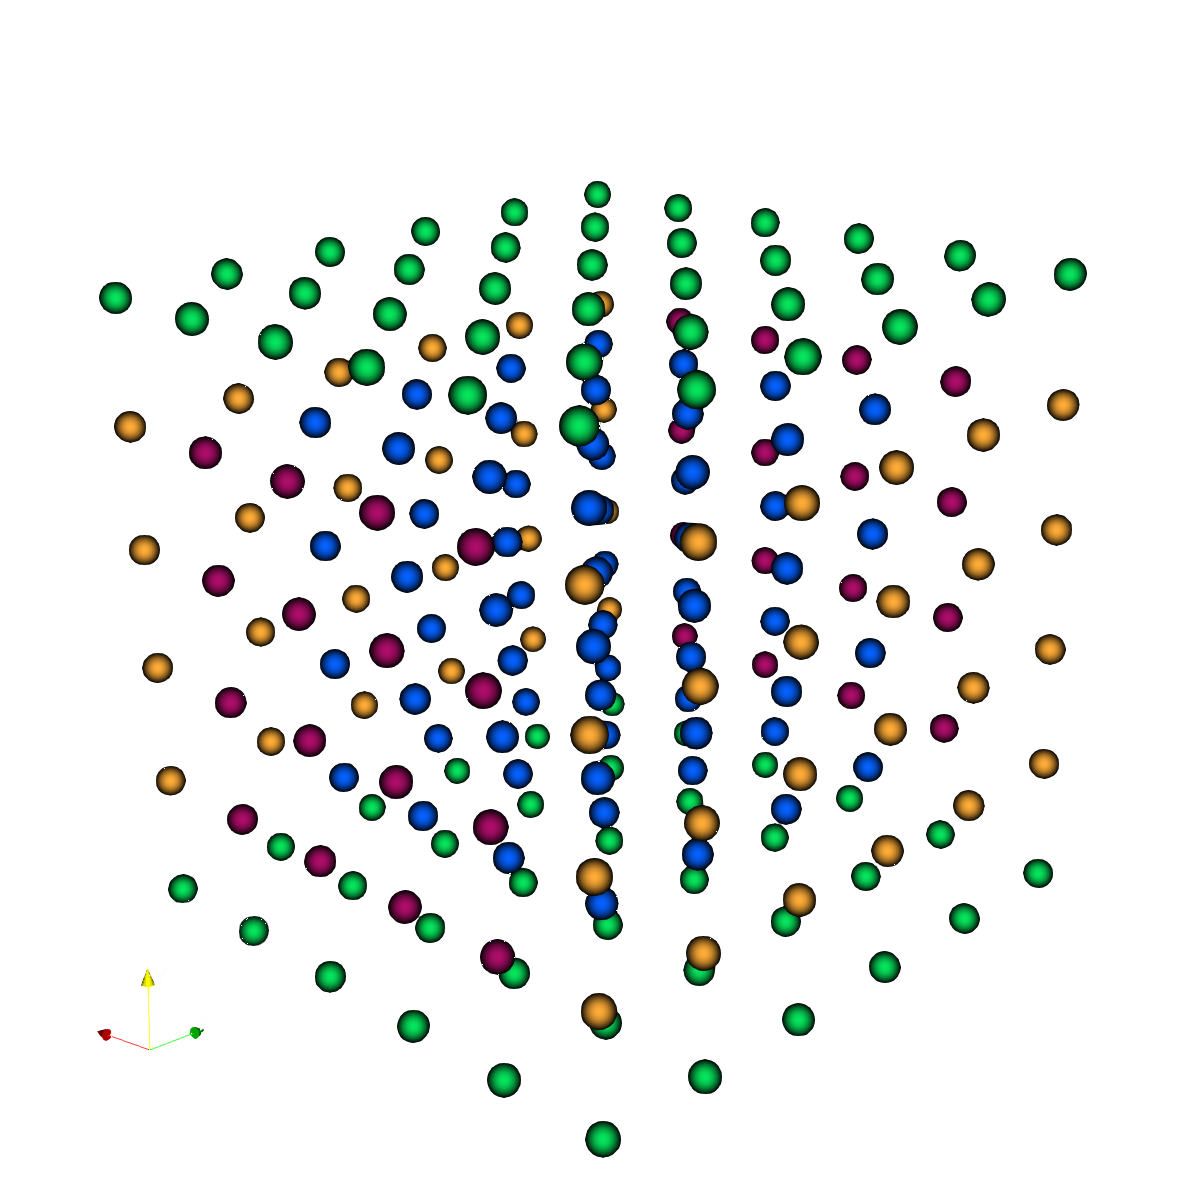
\includegraphics[width=0.6\linewidth]{group_rainbow.png}
  \end{center}
  \caption{The collision operator and applying boundary conditions are mutually exclusive.
  Here we see how different compute passes handle different parts of the domain.
Green ($xz$ faces) and orange ($yz$ faces) are slip boundaries.
Red ($xy$ faces) enforces the Dirichlet boundary conditions.
Blue (internal) gets the collision operator or specular slip boundary 
depending on the cell type.}
\end{figure}

\begin{figure}
  \begin{center}
    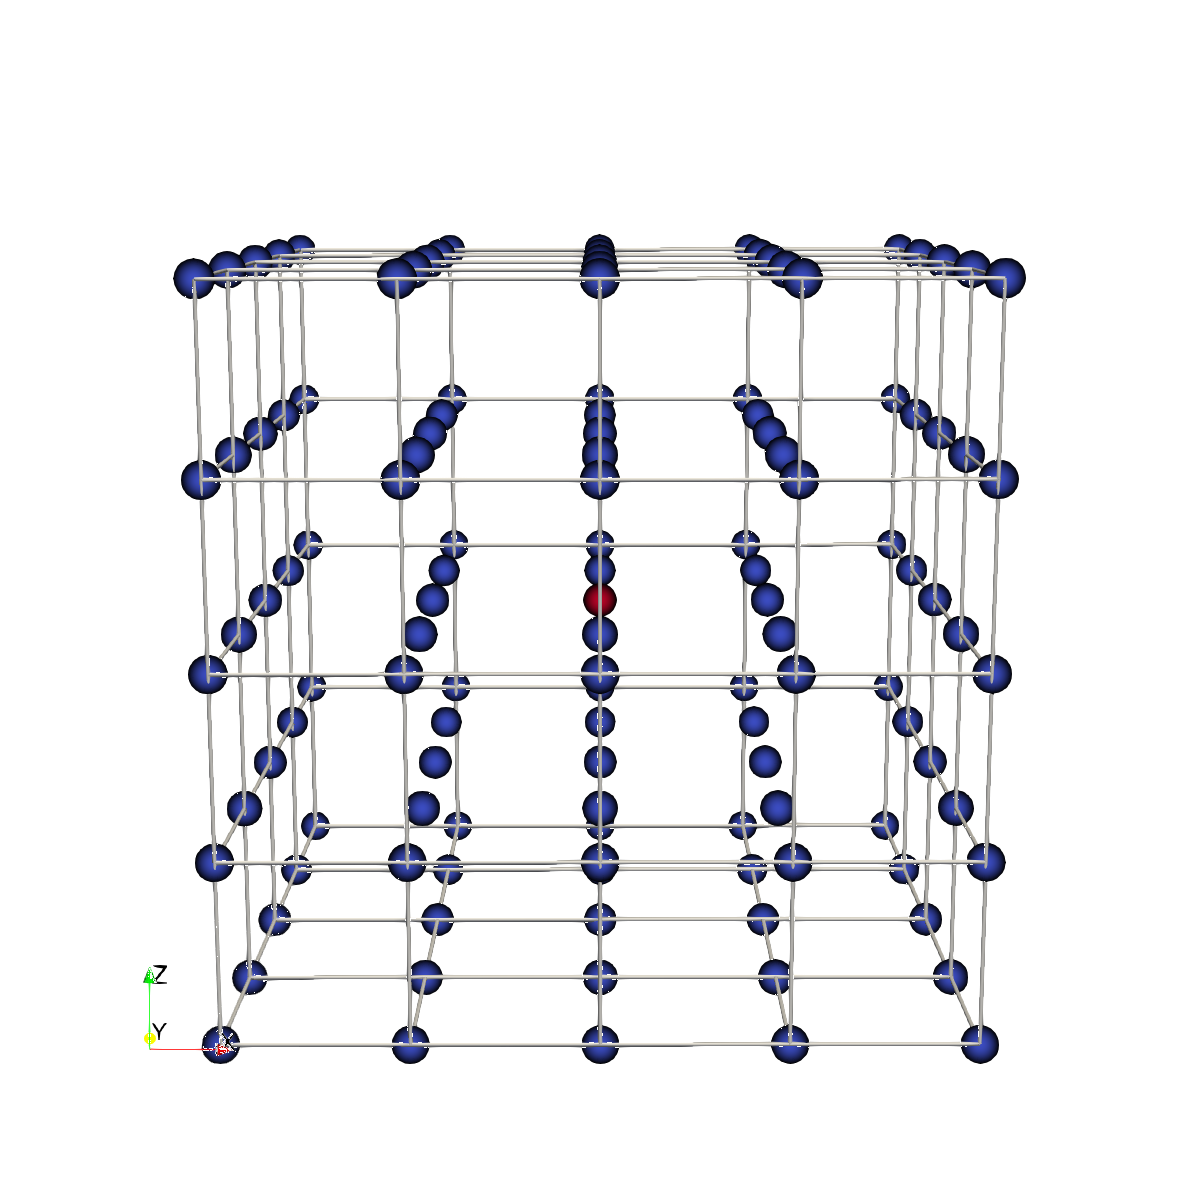
\includegraphics[width=0.4\linewidth]{stream_0.png}
    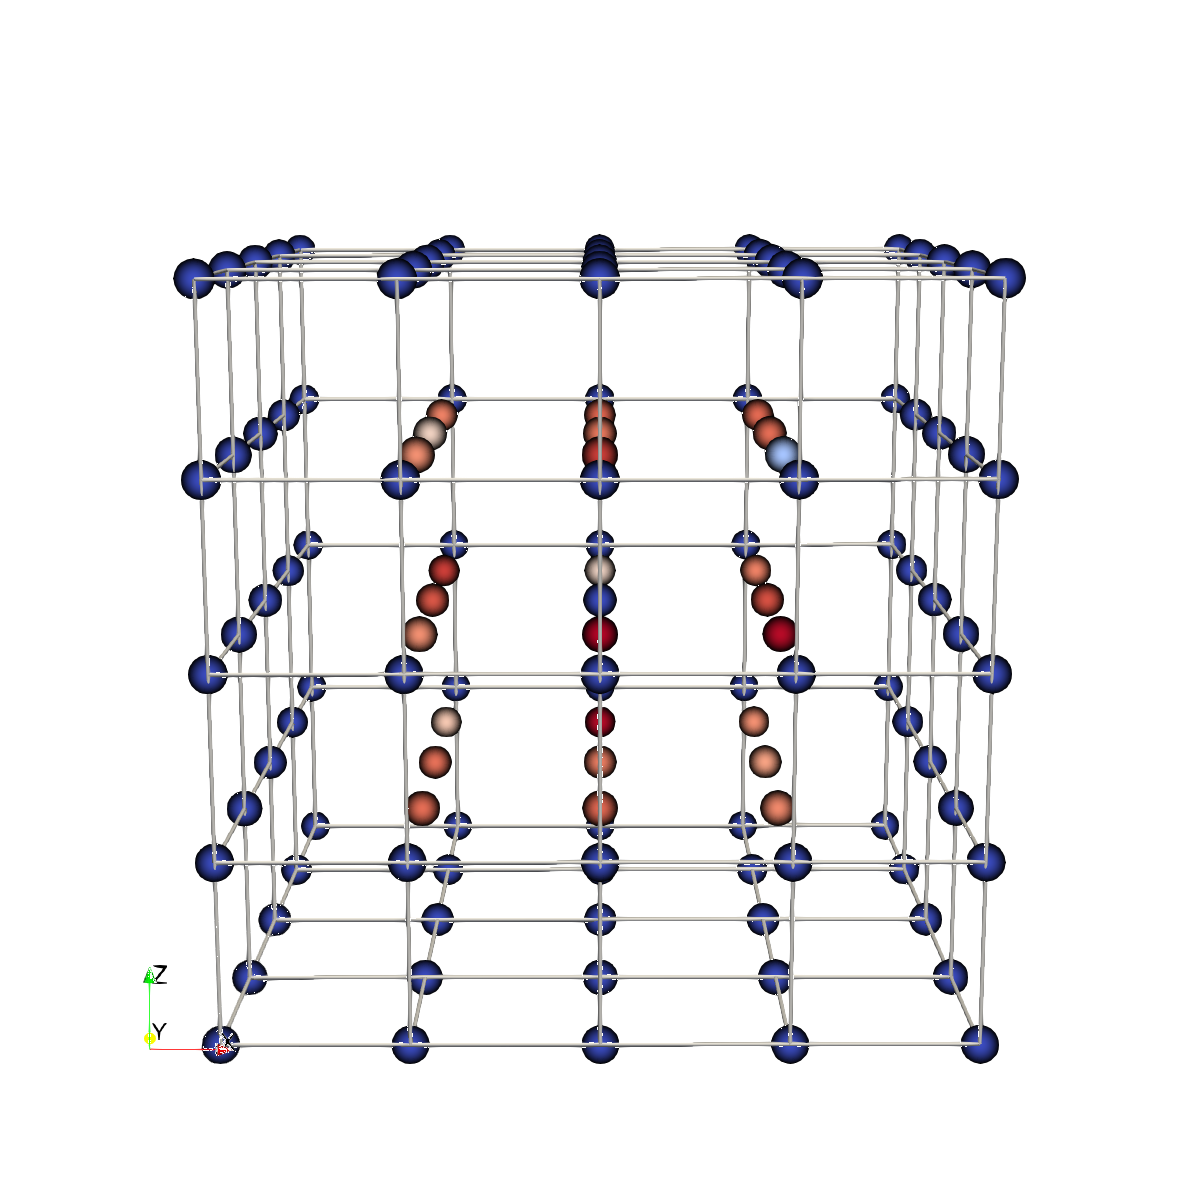
\includegraphics[width=0.4\linewidth]{stream_1.png}

    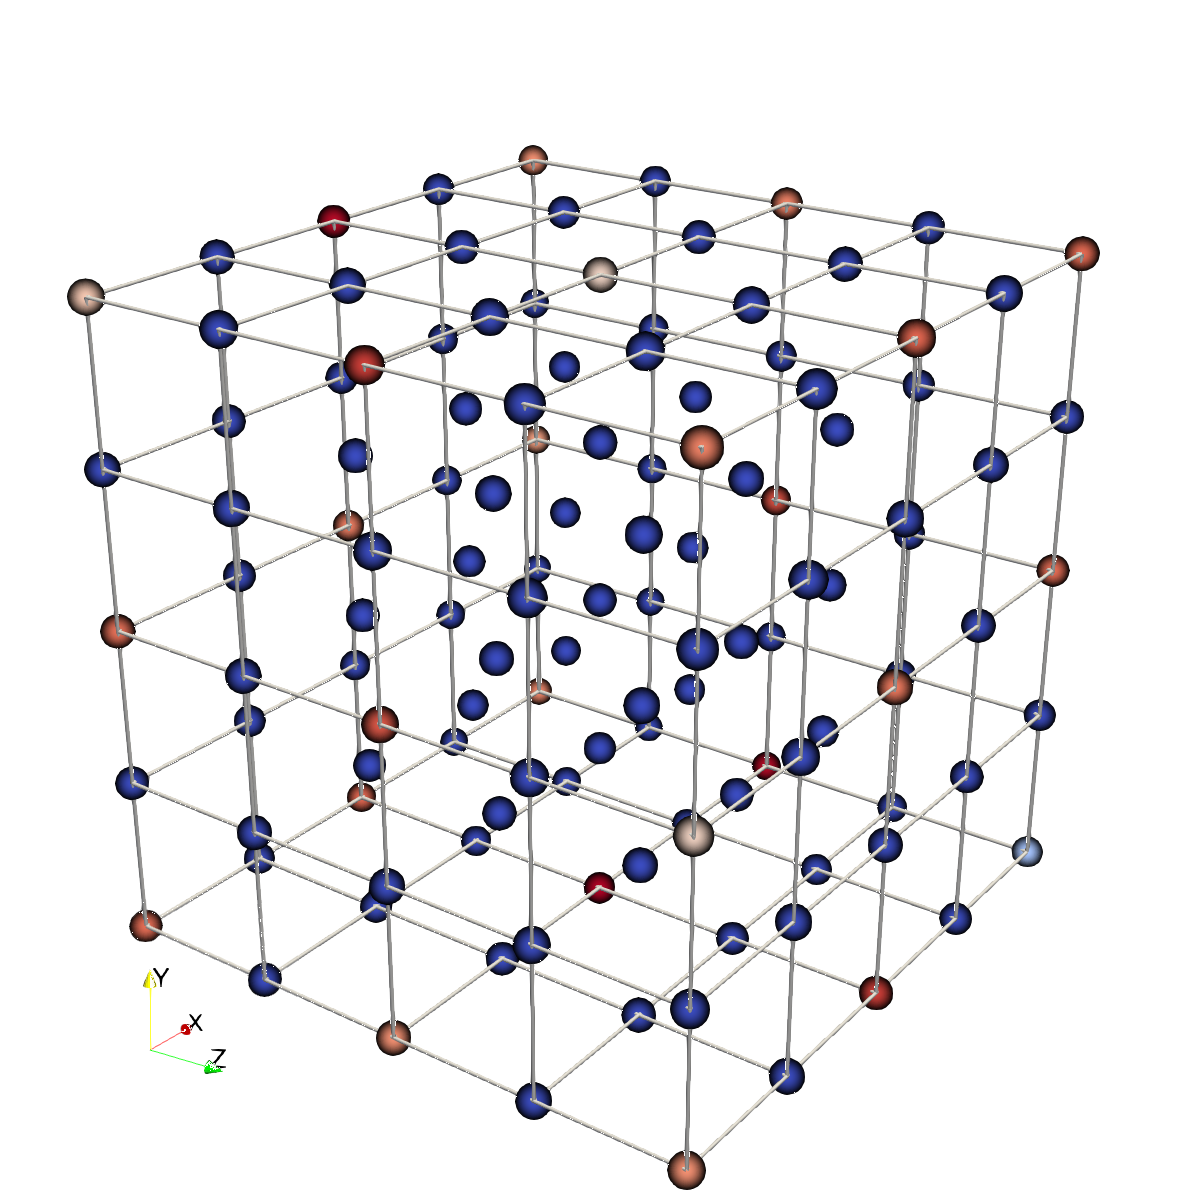
\includegraphics[width=0.6\linewidth]{stream_2.png}
  \end{center}
  \caption{Stream example}
\end{figure}

\begin{figure}
  \begin{center}
    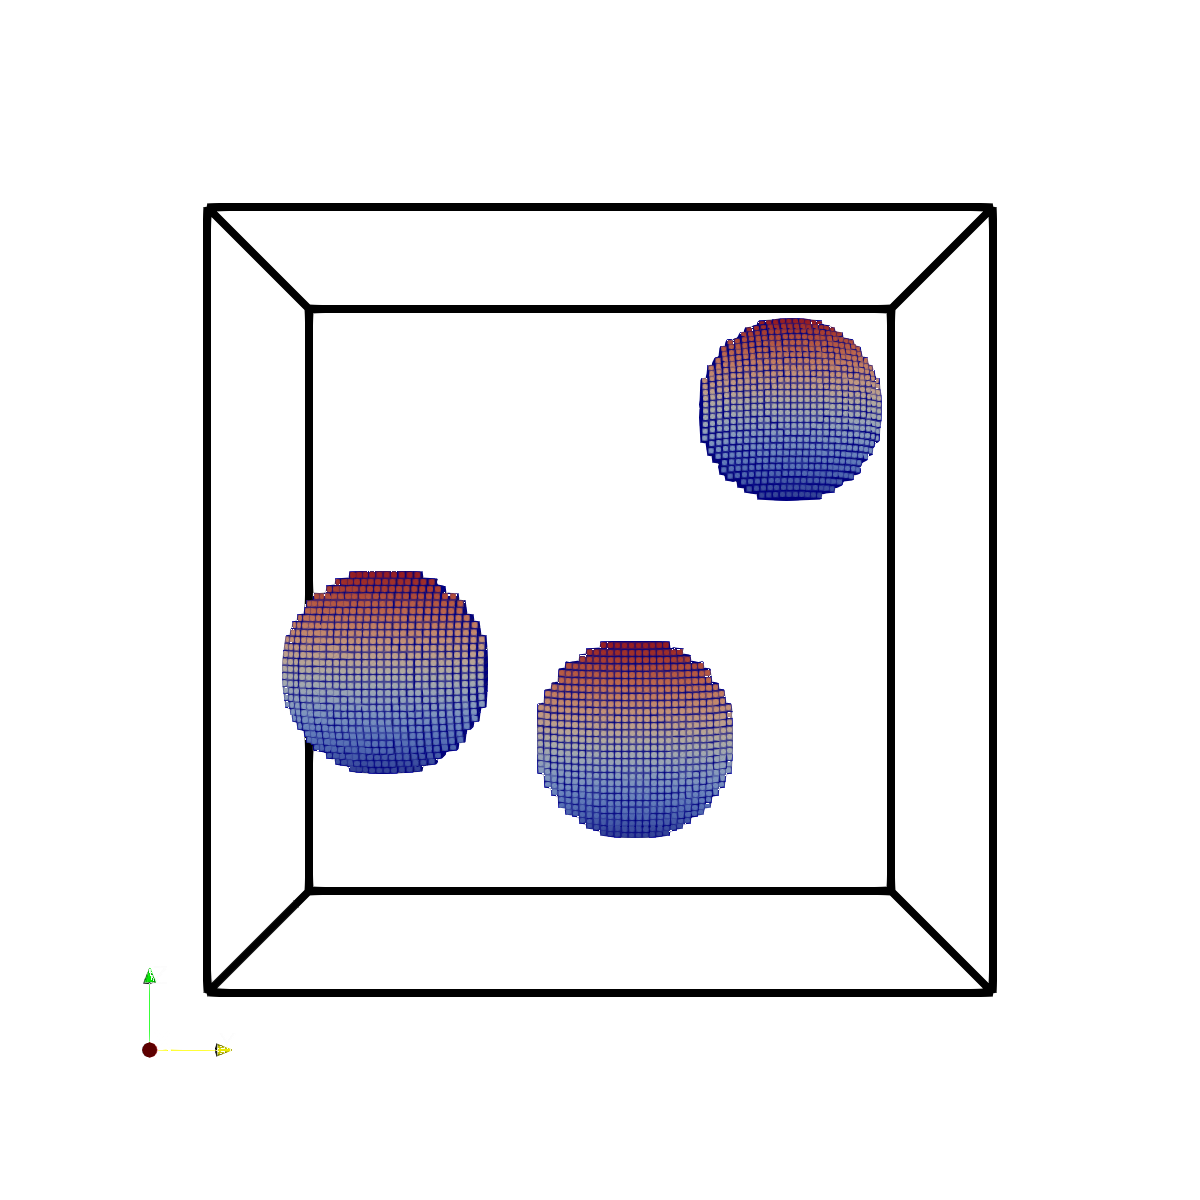
\includegraphics[width=\linewidth]{specular.png}
  \end{center}
  \caption{Specular Slip Boundaries.
For now we can add spheres, here we see those cells colored by the z component of the normal.}
\end{figure}
